\documentclass[conference]{IEEEtran}
\IEEEoverridecommandlockouts

\usepackage{amsmath,amssymb}
\usepackage{graphicx}
\usepackage{booktabs}
\usepackage{array}
\usepackage{float}
\usepackage{cite}
\usepackage{url}
\usepackage{xcolor}
\usepackage{microtype}
\usepackage[colorlinks=true,linkcolor=blue,citecolor=blue,urlcolor=blue]{hyperref}
\usepackage{CJKutf8}

\graphicspath{{figures/}}
\setlength{\textfloatsep}{5pt plus 1pt minus 1pt}
\setlength{\floatsep}{4pt plus 1pt minus 1pt}
\setlength{\intextsep}{4pt plus 1pt minus 1pt}
\setlength{\abovecaptionskip}{3pt}
\setlength{\belowcaptionskip}{0pt}

\title{CREATE: 基于训练证据的闭环奖励编辑智能体}
\author{\IEEEauthorblockN{匿名作者}\IEEEauthorblockA{匿名投稿}}

\begin{document}
\begin{CJK}{UTF8}{gbsn}
\maketitle

% ==================== 摘要 ====================
\begin{abstract}
评估语言模型生成的奖励函数需要完整的强化学习运行，然而大多数奖励搜索方法仅将该运行用于排序或替换候选方案。我们提出\textbf{CREATE}，一个基于训练证据的闭环奖励编辑智能体（\textbf{C}losed-loop \textbf{R}eward \textbf{E}diting \textbf{A}gent with \textbf{T}raining \textbf{E}vidence），它将每次运行视为对当前奖励谱系进行自我修复的一次观测。此处的"奖励自我演化"指的是语言模型权重固定不变，但奖励代码、诊断记忆和存档的优胜解在外部训练反馈下不断演化。CREATE 将原生任务结果与组件激活和幅度统计相结合，将诊断和编辑记录在持久记忆中，并施加一次严重性门控的干预，同时由最佳存档防止性能回退。在离散和连续 Gymnasium 任务上，CREATE 修复了所有测试的初始失败谱系，且选定的奖励在独立测试种子上仍然有效。消融实验表明，结构化证据和受限修订是共同重要的；追踪记录揭示了 L1 尺度修正和 L2 结构重构。这些结果支持通过闭环诊断和有界修复实现智能体的奖励自我演化。
\end{abstract}

\begin{IEEEkeywords}
强化学习，奖励设计，大语言模型，语言智能体，奖励自我演化，基于学习的控制
\end{IEEEkeywords}

% ==================== 1. 引言 (翻译自最终稿) ====================
\section{引言}
奖励设计将任务目标转化为强化学习策略所优化的信号。在实践中，这是一个调试循环：编写奖励函数，训练策略，检查行为，然后修订奖励。策略训练是其中代价最高的步骤，但其输出远不止一个分数。组件激活揭示了不可达的奖励项，幅度占比暴露了占主导地位的项，episode 结果区分了任务失败与奖励利用。这些测量补充了基于回报的标准 RL 视角。我们的公式受奖励塑形失败和更广泛的奖励误设问题启发。

具有代码能力的大语言模型可以将任务描述转化为可执行的稠密奖励函数。Text2Reward 强调可解释的奖励程序，而 Eureka 使用进化搜索与奖励反思。后来的系统加入了动态轨迹反馈、偏好反馈或智能体树搜索。这些方法主要关注"哪个候选方案应该存活"。我们则提出一个互补的问题：\emph{在训练当前奖励函数的过程中观察到所有信息之后，下一步应该修改什么？}

我们用 \textbf{CREATE} 来回答这个问题。CREATE 将每次完成的策略训练运行转化为一次观测，诊断出一个主要失败原因，并对当前奖励谱系施加一次有界操作。持久记忆为诊断提供条件；训练器和环境执行选定的编辑；最佳存档保护先前的解决方案。因此，"智能体"指的是一个闭环的观测--记忆--操作--转移循环，而不仅仅是重复的大语言模型调用。我们在精确的产物层面使用\emph{自我演化}：大语言模型权重保持不变，而奖励谱系通过外部评估的、记忆条件下的自我修复不断演化。

综上所述，本文将奖励设计重新定义为策略训练时间尺度上的智能体自我修复。它将用于学习的生成奖励与用于评估的原生目标分离，并使每次经过验证的 $R_t\!\rightarrow\!R_{t+1}$ 转移成为受控奖励自我演化的一步。我们在两个控制基准上通过预算匹配搜索、机制消融、独立测试episode和证据级案例来测试这一闭环。

% ==================== 2. 相关工作 (翻译自最终稿) ====================
\section{相关工作}

\subsection{奖励规范与误设}
奖励塑形可以加速学习，但只有受限的变换才能保持最优策略。逆奖励设计则将指定的目标视为关于不完美设计者的证据，并推理预期目标。这两条路线都促使我们将训练中优化的信号与用于评判行为的目标分离。CREATE 实现了这种分离：策略优化生成的奖励代码，而一个未修改的原生评估器则提供智能体的外部结果信号。

\subsection{基于大语言模型的奖励合成与搜索}
Language to Rewards 将任务描述映射为稠密的机器人奖励程序，Text2Reward 强调可执行和可解释的奖励代码。Eureka 将代码生成与进化搜索和奖励反思相结合。CARD 通过动态轨迹反馈增强修订；REvolve 引入人类偏好反馈；RF-Agent 将奖励构建组织为语言智能体树搜索。这些系统表明反馈可以改善生成，但候选方案选择和广泛重新生成可能掩盖了哪个奖励机制导致了下一个结果。CREATE 刻意以深度为导向：它保持一个谱系，识别一个主要失败，并将下一次昂贵的训练运行用于一个有界、可审计的干预。

\begin{figure*}[t]
\centering
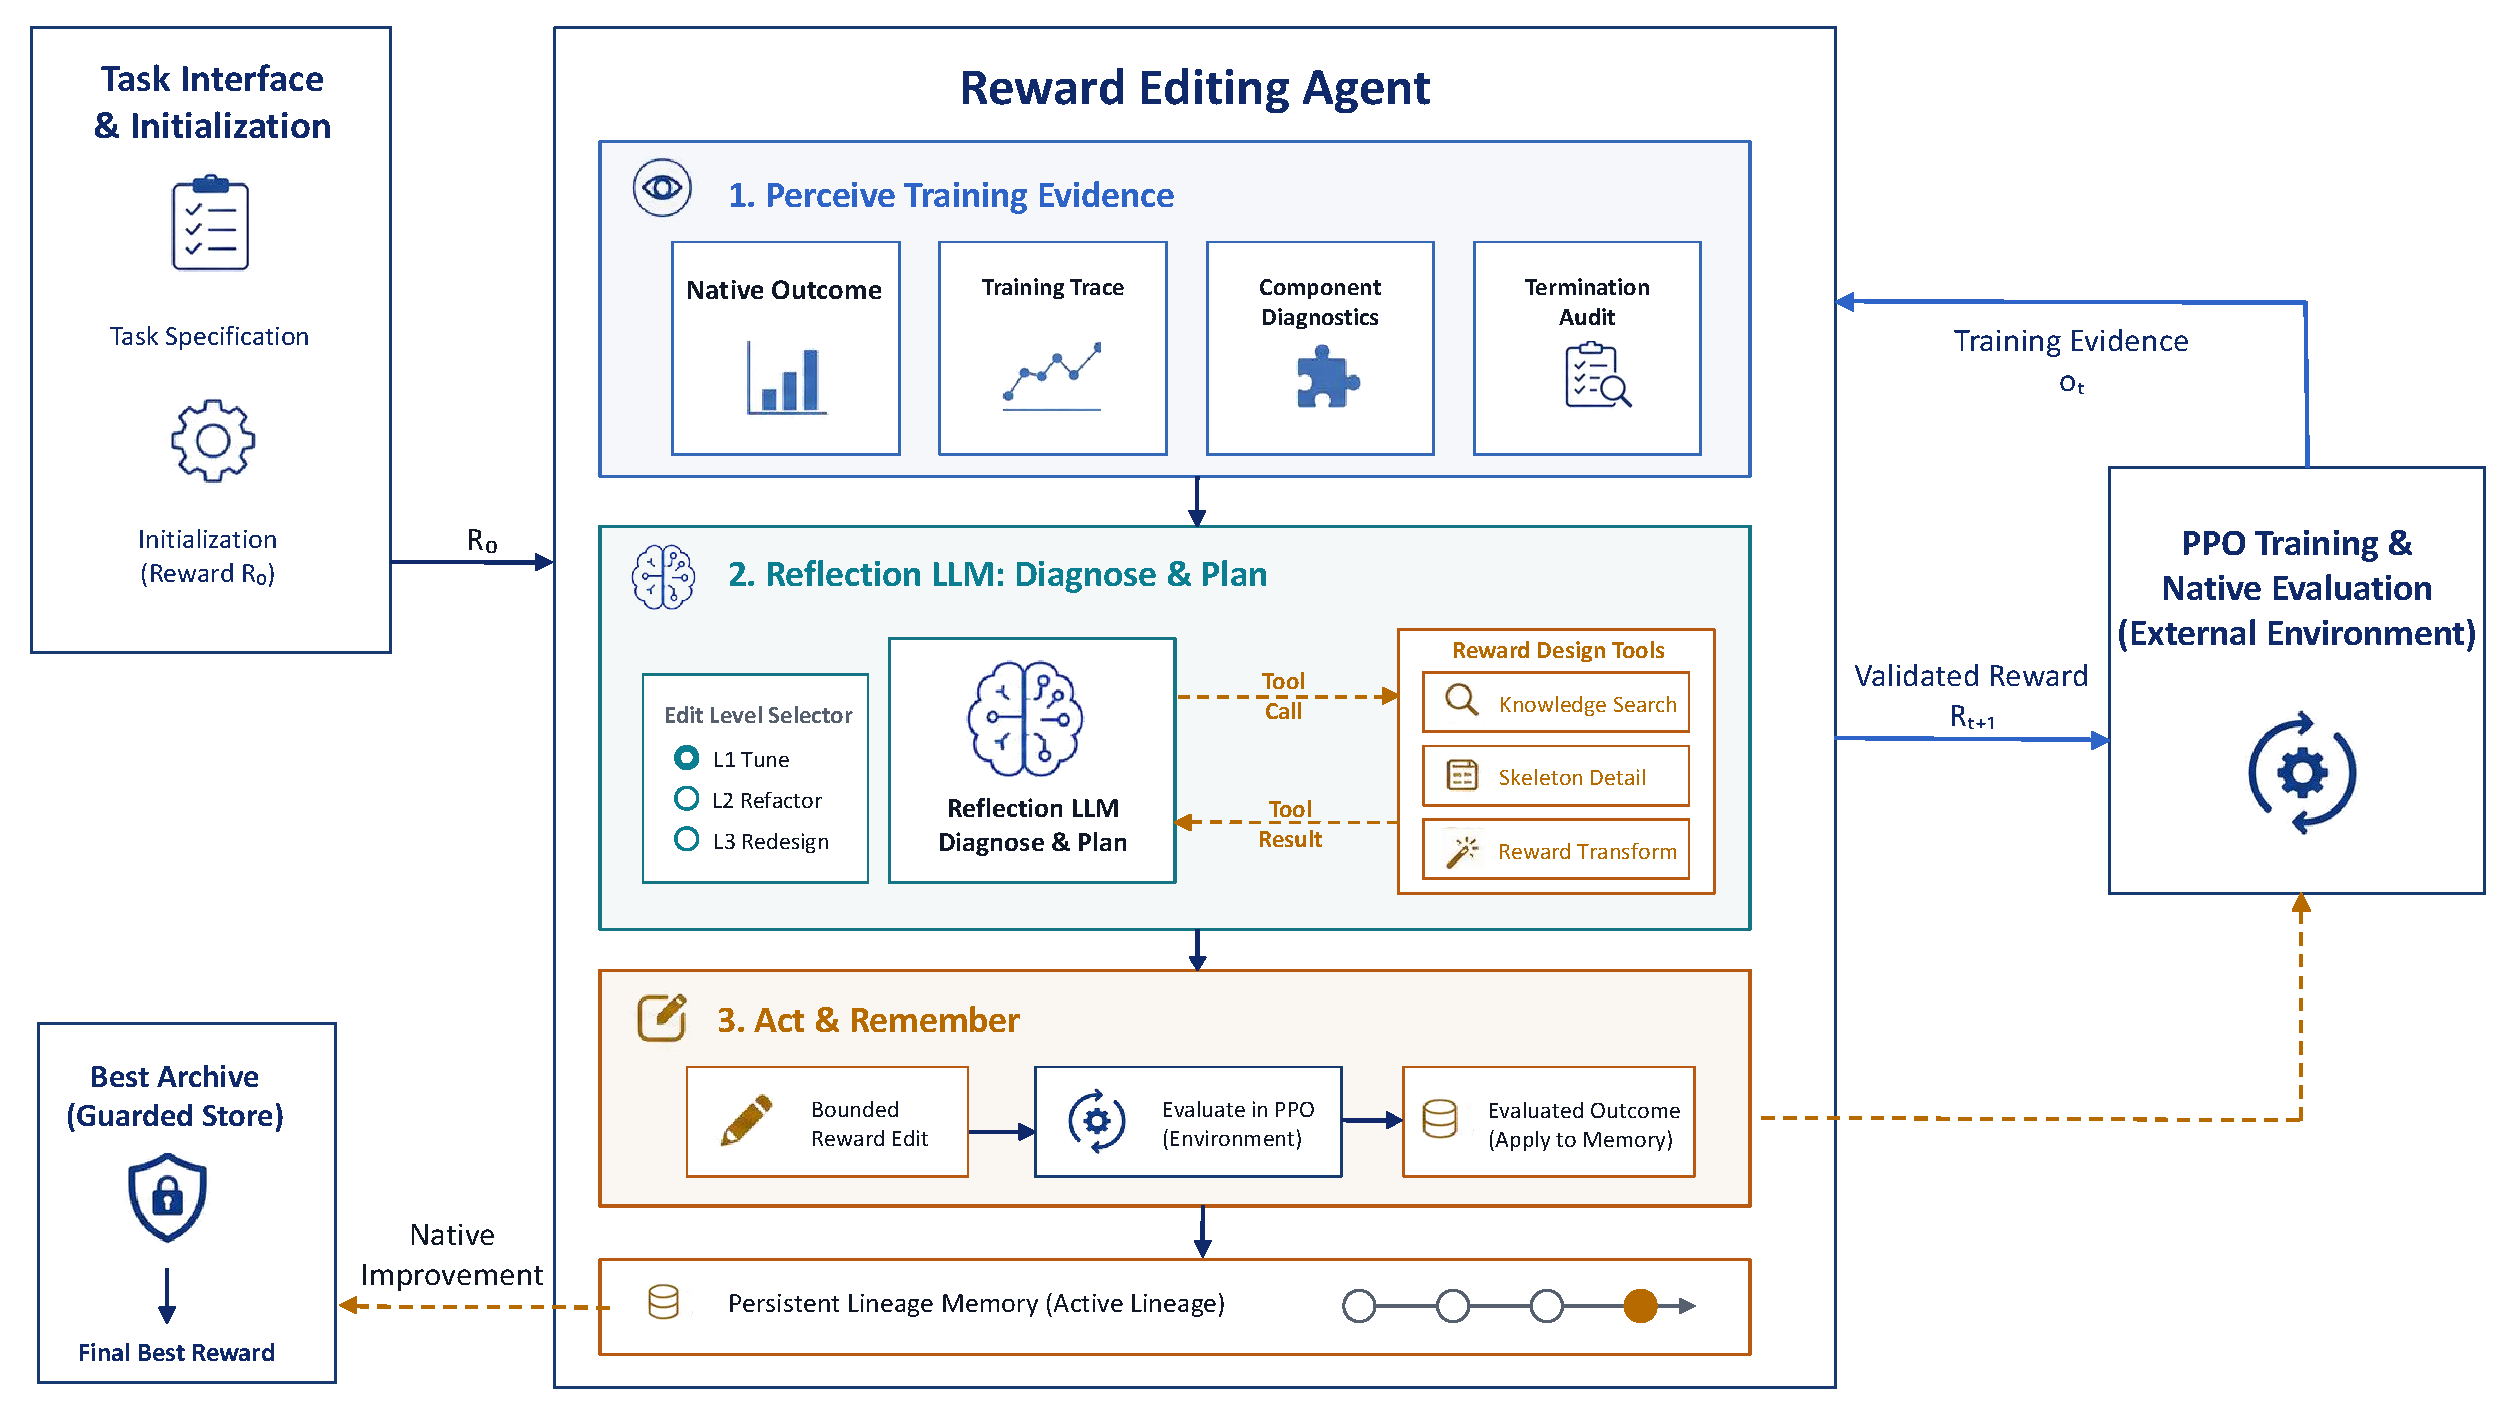
\includegraphics[width=0.98\textwidth]{cretae_framework.pdf}
\caption{CREATE 的闭环奖励修复循环。任务初始化产生 $R_0$。PPO 训练和原生评估返回训练轨迹和 $J_t$。智能体诊断一个失败，应用 L1/L2/L3 单一目标修复，将转移记录在持久记忆中，验证 $R_{t+1}$，并仅在原生性能提高时更新最佳存档。}
\label{fig:framework}
\end{figure*}

\subsection{反馈驱动的语言智能体}
ReAct 通过将语言推理与获取外部反馈的操作交织来建立观测--推理--操作模式。Reflexion 展示了存储的语言反馈如何在不更新模型权重的情况下改变后续决策。Voyager 将迭代环境反馈、自我验证和持久技能库结合起来。CREATE 在不同的时间尺度上采纳这些功能性智能体属性：一次操作编辑一个奖励程序，一次环境转移是一次完整的策略训练和原生评估运行。其记忆存储假设、编辑、预测和结果，而不仅仅是对话历史。

\subsection{诊断驱动的奖励精化}
最近的诊断驱动奖励精化将奖励失败视为调试，并强调有用的诊断词汇取决于任务结构。CREATE 通过一个完全指定的控制接口来补充这个方向：组件级测量定位失败；严重性门控限制了 L1/L2/L3 操作空间；程序检查在训练前拒绝无效编辑；最佳存档保护返回的解。因此，区分性主张不是大语言模型可以修订奖励函数，而是训练证据、有界操作、持久状态和外部转移共同形成一个可审计的、自我修复的奖励编辑智能体。

% ==================== 3. CREATE 方法 (翻译自最终稿) ====================
\section{CREATE}

\subsection{任务接口与智能体状态}
CREATE 每次奖励评估完成后执行一次操作，而非每个环境步长执行一次。在第 $t$ 次迭代中，策略学习器和原生评估器产生一次观测；奖励修复智能体随后选择下一个奖励程序。表~\ref{tab:agent} 总结了贯穿此决策周期的状态。

\begin{table}[t]
\caption{CREATE 奖励修复决策接口。}
\label{tab:agent}
\centering
\scriptsize
\setlength{\tabcolsep}{3.1pt}
\begin{tabular}{p{0.16\columnwidth}p{0.39\columnwidth}p{0.35\columnwidth}}
\toprule
状态元素 & 实现 & 在决策周期中的作用 \\
\midrule
观测 & 原生结果加上奖励组件统计 & 定位当前失败 \\
记忆 & 先前的奖励、诊断、编辑和结果 & 用谱系历史为下一个决策提供条件 \\
操作 & L1 调节、L2 重构或例外 L3 重新设计 & 限制正在测试的更改 \\
转移 & 通过新的策略训练运行执行编辑后的奖励 & 获得外部反馈 \\
存档 & 迄今观察到的最佳奖励--策略对 & 返回优胜者而非最后一次编辑 \\
\bottomrule
\end{tabular}
\end{table}

令智能体状态为
\begin{equation}
x_t=(R_t,M_t,A_t^\star),
\label{eq:state}
\end{equation}
其中 $R_t$ 是当前活跃的奖励程序，$M_t$ 是其谱系记忆，$A_t^\star$ 是迄今观察到的最佳奖励--策略对。策略训练使用生成的奖励，
\begin{equation}
(\pi_t,T_t)=\operatorname{Train}(\mathcal{E},R_t;B),
\label{eq:train}
\end{equation}
但策略质量仅通过未修改的原生目标来衡量：
\begin{equation}
J_t=\frac{1}{N}\sum_{i=1}^{N}\sum_{k=0}^{H_i-1}
r_{\rm env}(s_k^i,a_k^i,s_{k+1}^i).
\label{eq:native}
\end{equation}
这防止了生成的奖励函数自我宣称成功。每个已完成的候选方案消耗相同的固定交互预算 $B$；经过 $n$ 次评估后，主要成本为 $C(n)=nB$。

\subsection{训练证据观测}
假设 $R_t=\sum_{j=1}^{m_t}r_{t,j}$ 具有命名组件。从训练轨迹中，CREATE 计算每个组件的激活率和幅度占比：
\begin{equation}
\alpha_{t,j}=\frac{\sum_k\mathbb{I}(|r_{t,j}^{(k)}|>\epsilon)}{L_t},
\quad
\rho_{t,j}=\frac{\sum_k|r_{t,j}^{(k)}|}
{\sum_{\ell,k}|r_{t,\ell}^{(k)}|+\epsilon}.
\label{eq:evidence}
\end{equation}
激活率暴露沉默或过于稀疏的项；幅度识别主导学习信号的项。连同原生回报、episode 长度、终止模式、奖励源代码和谱系历史，它们构成 $E_t=(T_t,D_t,M_t)$。

\subsection{诊断智能体与有界修复策略}
智能体将 $E_t$ 映射到一个可证伪的失败假设 $h_t$、目标组件 $j_t^\star$ 和操作级别 $z_t$。L1 调节权重或门控；L2 改变一个语义组件的数学形式；L3 仅在反复局部失败后重新设计分解。对于 L1 和 L2，
\begin{equation}
|\mathcal{K}^{\rm edit}_t|=1,\qquad
R_{t+1}=\mathcal{U}(R_t,h_t,j_t^\star,z_t).
\label{eq:update}
\end{equation}
决策记录刻意比自由形式的反思更加结构化。它必须识别测量到的症状，将该症状与一个奖励机制联系起来，陈述提议的干预，预测下一轮可观测的变化，并记录主要反风险。例如，一个激活率 $\alpha_{t,j}=0$ 的着陆奖励不会自动增加：如果 episode 在远离着陆区域处终止，诊断则应针对应使该事件可达的接近信号。这种区分防止了将稀疏成功项误判为缺陷项。

\subsection{奖励转移、记忆与最佳存档}
训练前，编辑后的程序会对照环境接口进行检查，在采样转移上执行，并被要求返回有限标量加上已命名的组件值。检查失败不会消耗策略训练；它将作为运行时观测返回给修复步骤。有效运行后，预测的行为和组件变化将对照新的 $D_{t+1}$ 和 $T_{t+1}$ 进行比较，并追加到记忆中。因此，记忆不仅用于保存文本，还用于测试先前假设是否被新策略支持、反驳或变得无关。

单一目标规则使下一次训练运行具有可解释性，尽管它不声称在随机 RL 下具有因果识别性。评估后，$M_t$ 记录完整转移，$A_t^\star$ 保留最大原生分数。循环在达到任务阈值或评估上限时停止。

% ==================== 4. 实验 (翻译自原始稿) ====================
\section{实验}

\subsection{实验设置与对比}
我们使用 Gymnasium 的 LunarLander-v3 和 BipedalWalker-v3 环境，通过 Stable-Baselines3 为每个奖励候选方案训练全新的 PPO 策略。每个条件包含五个独立的搜索谱系（种子 0--4）。当谱系的原生平均分数首次达到任务阈值或经过十次奖励评估后停止。表~\ref{tab:protocol} 总结了训练和评估设置。

\begin{table}[H]
\caption{每个奖励搜索谱系的实验协议。}
\label{tab:protocol}
\centering
\scriptsize
\setlength{\tabcolsep}{2.7pt}
\begin{tabular}{lccccc}
\toprule
任务 & 动作 & 步数 & 修复/测试 & 阈值 & 运行次数 \\
\midrule
LunarLander & 离散 & 1M & 20/100 & 200 & 5 \\
BipedalWalker & 连续 & 5M & 20/100 & 300 & 5 \\
\bottomrule
\end{tabular}
\end{table}

20 个修复 episode 使用固定种子；其原生分数和组件统计可供 CREATE 使用。选定后，返回的奖励在 100 个从未进入修复循环的独立测试种子上进行评估。生成的奖励在 PPO 训练期间被裁剪至 $[-20, 20]$，而原生评估器保持不变且未裁剪。

我们使用两个基线和两个机制消融。\emph{初始奖励}是单次生成，不进行修订。\emph{独立生成}将相同的十次评估预算用于十个不相关的候选方案，并保留最好的。\emph{粗粒度反馈}保留单一目标编辑，但仅向编辑器提供原生分数，移除组件定位。\emph{无约束修订}保留组件证据，但允许多个奖励机制同时更改，移除了 L1/L2/L3 层次结构和单一目标规则。因此，基线测试修复谱系是否有用，而消融测试它为什么有用。

\begin{table}[H]
\caption{LunarLander 基线和机制消融（每组五个谱系）。}
\label{tab:baseline}
\centering
\scriptsize
\setlength{\tabcolsep}{3.1pt}
\begin{tabular}{lcccc}
\toprule
条件 & 证据 & 编辑范围 & 成功率 & 平均分数 \\
\midrule
初始奖励（基线）& -- & -- & $0/5$ & $-2.21$ \\
独立生成（基线）& -- & 新奖励 & $0/5$ & $-0.74$ \\
粗粒度反馈（消融）& 分数 & 单一目标 & $2/5$ & $134.97$ \\
无约束（消融）& 组件 & 多目标 & $0/5$ & $114.21$ \\
CREATE & 组件 & 单一目标 & $\mathbf{5/5}$ & $\mathbf{228.98}$ \\
\bottomrule
\end{tabular}
\end{table}

每个条件在任务内使用相同的修复种子，独立测试种子仅在选择后使用。每组五个谱系，我们展示所有结果及其观测范围，而非依赖大样本检验。我们仅比较 CREATE 和独立生成的训练成本，因为它们的完整轨迹使用相同的评估预算。独立候选方案可以并行运行，而 CREATE 的编辑是顺序的；因此成本比较涉及策略训练次数，而非实际耗时。

表~\ref{tab:baseline} 将基线失败与机制失败分开。单次生成基线表明仅靠生成是不够的，预算匹配基线表明简单生成更多不相关的奖励无法恢复缺失的信号。粗粒度反馈偶尔成功，因此迭代编辑确实具有有用的搜索能力，但其三次失败表明标量结果无法可靠地识别应更改的内容。相反，无约束修订接收正确的证据，但由于多个机制可以同时移动而失去了归因。CREATE 将定位与有界操作相结合，分别经过 8、10、2、4 和 3 次策略训练达到阈值，总共 27 次训练。

\subsection{整体结果与修复行为}
图~\ref{fig:performance} 展示了带有预算限制的 LunarLander 搜索。CREATE 的最佳历史原生分数随着证据的积累而提高，每个谱系都越过了阈值，而独立生成始终低于阈值。独立种子测试分数与修复分数接近，表明选择并非仅仅利用固定的修复 episode。

\begin{figure}[H]
\centering
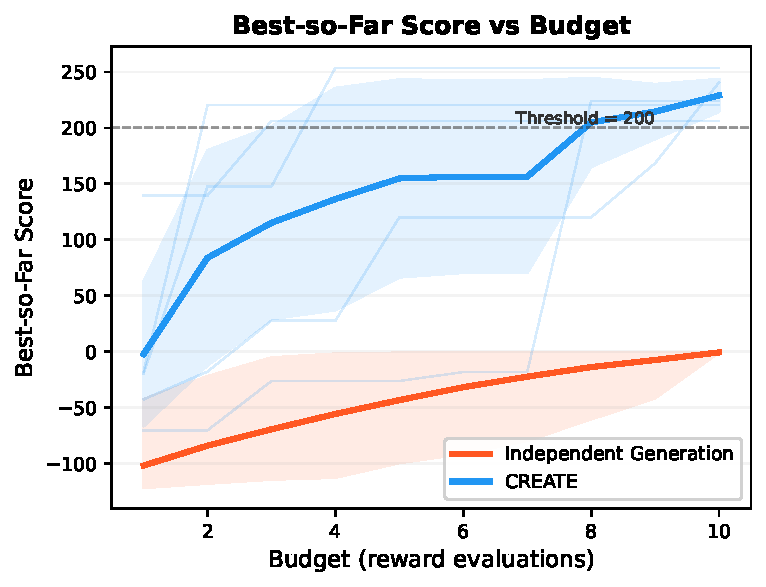
\includegraphics[width=\columnwidth]{performance_curve.pdf}\\[-2pt]
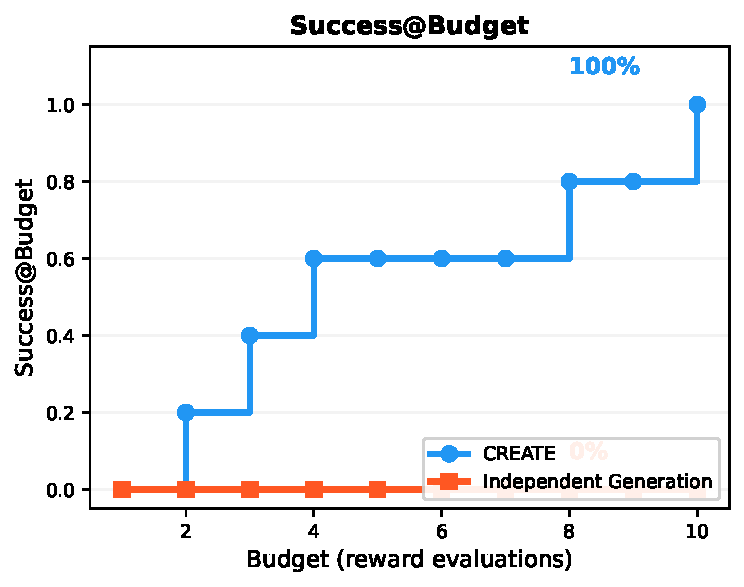
\includegraphics[width=0.485\columnwidth]{success_by_budget.pdf}\hfill
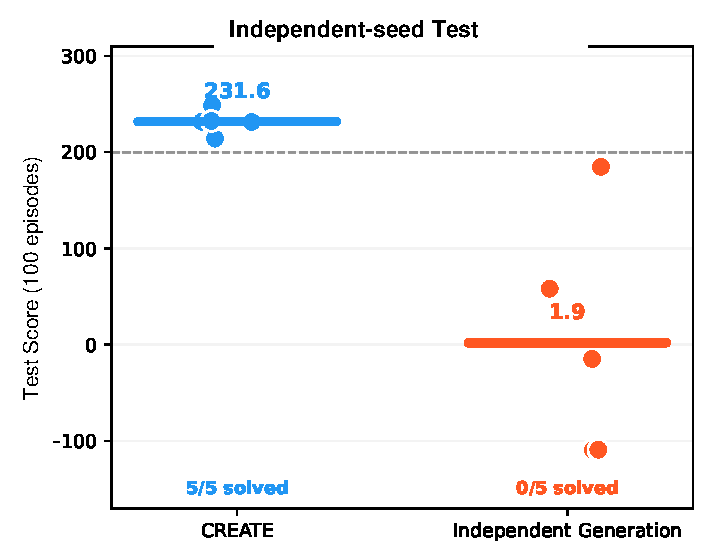
\includegraphics[width=0.485\columnwidth]{independent_test_scatter.pdf}
\caption{LunarLander 上的预算奖励搜索。(a) 中的阴影跨越五次运行；(b) 报告其存档超过 200 的比例；(c) 比较选定奖励的修复分数和独立测试分数。每一点都来自存档的原生奖励评估。}
\label{fig:performance}
\end{figure}

修复历史也揭示了两种互补的改进模式。L1 编辑保留组件的数学形式并修正其尺度；例如，降低过度加权的进度项将一个月球着陆器谱系从 $-29.48$ 提升至 $120.02$。L2 编辑在缩放无法帮助时改变奖励几何：将不可达的乘法着陆项替换为独立可达的部分信用因子，将另一个谱系从 $-17.90$ 提升至 $220.24$。因此，CREATE 不仅仅是在爬分数曲线。它首先判断缺陷是参数性的还是结构性的，然后在相应级别上修改一个组件。

\begin{table}[H]
\caption{BipedalWalker 上的连续控制迁移。"跨越"是第一个达到原生阈值 300 的奖励。}
\label{tab:bipedal}
\centering
\scriptsize
\setlength{\tabcolsep}{4.0pt}
\begin{tabular}{ccccc}
\toprule
种子 & 初始 & 跨越 & 增益 & 评估次数 \\
\midrule
0 & 270.71 & 318.32 & $+47.60$ & 2 \\
1 & 280.50 & 313.46 & $+32.96$ & 2 \\
2 & 272.07 & 307.92 & $+35.85$ & 2 \\
3 & 289.99 & 311.12 & $+21.14$ & 2 \\
4 & 103.03 & 304.92 & $+201.90$ & 3 \\
\bottomrule
\end{tabular}
\end{table}

表~\ref{tab:bipedal} 测试了相同的修复逻辑是否从离散动作迁移到连续控制。四个初始奖励已经接近阈值，因此它们的增益显示了保守的精化。困难的种子提供了更强的机制检验：前向进展加稳定性仅达到 103.03，第一次有界精化将其提升至 264.39，添加能量使用组件后超过 300。综合来看，这些轨迹表明 CREATE 可以保留有用的奖励骨架，同时补充缺失的控制信号。

\subsection{机制消融}
图~\ref{fig:ablation} 将选定分数质量与成功可靠性分开。粗粒度反馈在 2/5 的搜索中成功，表明仅靠迭代编辑可以奏效，但没有组件定位是不可靠的。无约束修订尽管接收了结构化证据，却在 0/5 中成功：当一次操作可以同时重写多个机制时，观测质量是不够的。CREATE 在 27 次策略训练中实现了全部五次成功，而独立生成使用的固定预算为 50 次训练。

\begin{figure}[H]
\centering
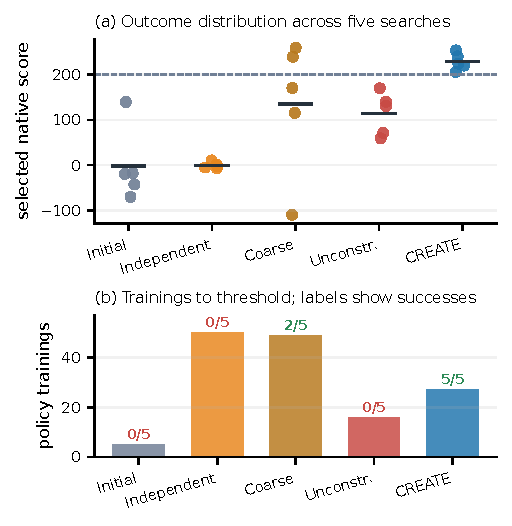
\includegraphics[width=\columnwidth]{ablation.pdf}
\caption{LunarLander 机制消融。(a) 中短横线为五次运行的平均值。(b) 面板再现了存档的实际计数视图；其消融计数是描述性的，而非效率比较，因为相应的迭代轨迹不完整。}
\label{fig:ablation}
\end{figure}

独立候选方案是可并行的，而 CREATE 的编辑是顺序的。因此，27 对 50 是达到成功所需的环境交互次数比较，而非实际耗时的声明。独立基线还使用了更简单的初始化提示，联合无约束消融未单独分离编辑层次结构和编辑范围。我们不对两个消融的实际训练计数进行比较，因为它们存档的迭代轨迹不完整，因此不支持对等的效率声明。

\subsection{证据引导的修复案例研究}
图~\ref{fig:case} 跟踪了 LunarLander 种子 0。仅看总分似乎不稳定。组件证据揭示了原因。在第 7 次迭代中，\texttt{approach\_shaping} 是唯一激活的接近项，但策略在 19/20 个 episode 中提前终止，从未激活着陆或稳定着陆项。存储的诊断预测差分距离信号过于嘈杂，并提议用基于状态的 \texttt{landing\_proximity} 项进行 L2 替换。下一轮运行越过阈值，并使着陆相关项变为可观测。

轨迹在第 8 次迭代（首次越过阈值）处结束，最佳存档返回该奖励。其记录形成了一条可检验的五链环节。测量证据为分数 $-388.67$，平均 episode 长度 109.5，19/20 提前终止，着陆事件不活跃。诊断将这些症状归因于微弱、嘈杂的差分接近信号。L2 操作仅将该组件替换为带有门控的、基于状态的着陆接近项。训练前，记录预测 episode 长度增加、着陆项可达和更高的原生分数。下一轮运行达到 224.21，着陆接近项几乎在每步都活跃，着陆和稳定着陆项变为可观测。因为预测和反风险在结果之前就已存储，该轨迹可以在不依赖事后叙述的情况下进行审计。

\begin{figure}[H]
\centering
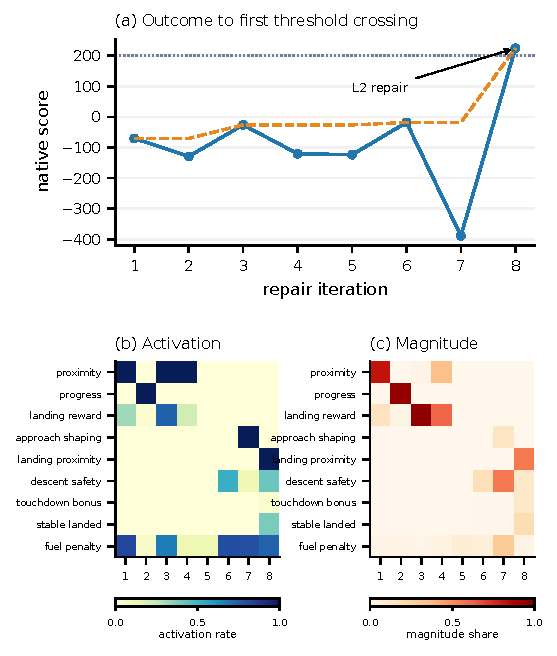
\includegraphics[width=\columnwidth]{repair_case.pdf}
\caption{一次可审计的修复。(a) 原始原生分数仅显示到第一次越过阈值。(b)--(c) 显示每个训练运行中哪些命名的奖励组件活跃并占主导地位；它们分别用颜色编码激活率和幅度占比。缺失的格子表示不存在或不活跃的组件，因此在解释时也需要使用存档的奖励源代码和 episode 结果。}
\label{fig:case}
\end{figure}

\subsection{数据来源与报告范围}
图~\ref{fig:performance}、\ref{fig:ablation} 和 \ref{fig:case} 中的每个分数都来自存档的原生评估记录。每个谱系还存储奖励源代码、episode 结果、组件统计、诊断和编辑级别，因此图表是可复现的。TensorBoard 验证 PPO 预算；跨候选方案比较使用公式~\eqref{eq:native} 中的共同原生评估器，因为塑形回报具有候选方案特定的尺度。

独立种子测试针对固定修复种子上的选择，而非新动态或任务转移。BipedalWalker 验证了连续动作，但四个初始奖励已接近阈值；因此种子 4 是更强的迁移样本，而 LunarLander 提供了更清晰的机制消融。

\section{讨论与结论}
核心发现是，一次失败的策略训练运行可以转化为用于自我修复和受控奖励演化的结构化观测。组件统计定位缺陷，原生评估防止自我评分，有界操作保持归因，记忆连接连续的编辑，存档保护优胜解。因此，CREATE 通过持久的智能体实现奖励程序的自我演化，而非底层大语言模型的自主适应。

证据仍然局限于 PPO、两个基准和每个任务五次搜索。提示匹配的基线、分解编辑消融、更多 RL 算法和更广泛的任务仍然是必要的。在此范围内，CREATE 将训练失败转化为结构化观测，并将每个测试谱系修复至其任务阈值。

\enlargethispage{5\baselineskip}
\fontsize{6.7}{7.1}\selectfont
\begin{thebibliography}{00}
\setlength{\itemsep}{-1.2pt}
\setlength{\parskip}{0pt}
\bibitem{sutton2018rl}
R. S. Sutton and A. G. Barto, \emph{Reinforcement Learning: An Introduction},
2nd ed. Cambridge, MA, USA: MIT Press, 2018.
\bibitem{ng1999policy}
A. Y. Ng, D. Harada, and S. Russell, ``Policy invariance under reward
transformations: Theory and application to reward shaping,'' in \emph{Proc.
ICML}, 1999, pp. 278--287.
\bibitem{hadfield2017inverse}
D. Hadfield-Menell, S. Milli, P. Abbeel, S. Russell, and A. Dragan, ``Inverse
reward design,'' in \emph{Advances in Neural Information Processing Systems},
vol. 30, 2017.
\bibitem{language2rewards}
W. Yu \emph{et al.}, ``Language to rewards for robotic skill synthesis,'' in
\emph{Proc. Conf. Robot Learning}, 2023, pp. 374--404.
\bibitem{text2reward}
T. Xie \emph{et al.}, ``Text2Reward: Reward shaping with language models for
reinforcement learning,'' in \emph{Proc. ICLR}, 2024.
\bibitem{eureka}
Y. J. Ma \emph{et al.}, ``Eureka: Human-level reward design via coding large
language models,'' in \emph{Proc. ICLR}, 2024.
\bibitem{card}
H. Sun, Y. Wu, H. Luo, J. Gu, and W. Xu, ``CARD: A large language model-driven
reward design framework via dynamic feedback for reinforcement learning,''
\emph{Knowledge-Based Systems}, vol. 326, p. 114065, 2025.
\bibitem{revolve}
R. Hazra, R. Moraes, S. Dasgupta, and J. Pajarinen, ``REvolve: Reward evolution
with large language models using human feedback,'' in \emph{Proc. ICLR}, 2025.
\bibitem{rfagent}
N. Gao, X. Zhang, X. Jiang, M. You, M. Zhang, and Y. Deng, ``RF-Agent:
Automated reward function design via language agent tree search,'' in
\emph{Advances in Neural Information Processing Systems}, vol. 38, 2025.
\bibitem{react}
S. Yao, J. Zhao, D. Yu, N. Du, I. Shafran, K. Narasimhan, and Y. Cao,
``ReAct: Synergizing reasoning and acting in language models,'' in
\emph{Proc. ICLR}, 2023.
\bibitem{reflexion}
N. Shinn, F. Cassano, E. Berman, A. Gopinath, K. Narasimhan, and S. Yao,
``Reflexion: Language agents with verbal reinforcement learning,'' in
\emph{Advances in Neural Information Processing Systems}, vol. 36, 2023.
\bibitem{voyager}
G. Wang, Y. Xie, Y. Jiang, A. Mandlekar, C. Xiao, Y. Zhu, L. Fan, and A.
Anandkumar, ``Voyager: An open-ended embodied agent with large language
models,'' \emph{arXiv preprint arXiv:2305.16291}, 2023.
\bibitem{wang2026diagnostic}
Y. Wang, Y. Tang, B. Liu, X. Liu, and D. Shang, ``When LLM reward design
fails: Diagnostic-driven refinement for sparse structured RL,'' \emph{arXiv
preprint arXiv:2605.28918}, 2026.
\bibitem{ppo}
J. Schulman, F. Wolski, P. Dhariwal, A. Radford, and O. Klimov, ``Proximal
policy optimization algorithms,'' \emph{arXiv preprint arXiv:1707.06347}, 2017.
\bibitem{sb3}
A. Raffin \emph{et al.}, ``Stable-Baselines3: Reliable reinforcement learning
implementations,'' \emph{J. Mach. Learn. Res.}, vol. 22, no. 268, pp. 1--8,
2021.
\end{thebibliography}

\end{CJK}
\end{document}
